% =============================================================================
%  FIVUCSAS — Poster variant: ACADEMIC / IEEE-CONFERENCE STYLE
%  A0 portrait, 2-column body, serif, conservative blue/black palette.
%  Compliant with Marmara CSE4198 Poster Preparation Guide §5.1:
%    Title · Logos (University + Faculty) · Group/Advisor ·
%    Problem · Contributions · Methods · Experiments · Conclusion.
%  Compile:  pdflatex poster.tex && pdflatex poster.tex
% =============================================================================
\documentclass[a0paper,portrait]{tikzposter}
\tikzposterlatexaffectionproofoff
\geometry{paperwidth=841mm,paperheight=1189mm}

\usepackage[utf8]{inputenc}
\usepackage[T1]{fontenc}
\usepackage{lmodern}   % serif default
\usepackage{microtype}
\usepackage{xcolor}
\usepackage{graphicx}
\graphicspath{{../../assets/}{./assets/}{./poster/assets/}}
\usepackage{fontawesome5}
\usepackage{qrcode}
\usepackage{tikz}
\usepackage{enumitem}
\usepackage{booktabs}
\usepackage{array}
\usetikzlibrary{positioning,calc,arrows.meta,backgrounds}

% ---------- IEEE-flavoured palette (conservative) ----------------------------
\definecolor{IEEEnavy}{HTML}{15376E}
\definecolor{IEEEblue}{HTML}{2B5CA0}
\definecolor{IEEEaccent}{HTML}{0F4C81}
\definecolor{IEEEgold}{HTML}{B58A2C}
\definecolor{IEEEred}{HTML}{B6202A}
\definecolor{IEEEink}{HTML}{0E1116}
\definecolor{IEEEgray}{HTML}{6E747A}
\definecolor{IEEElite}{HTML}{F4F6FA}
\definecolor{IEEErule}{HTML}{C7CCD3}

% ---------- Theme: clean filled title, minimal block styling -----------------
\definelayouttheme{IEEEStyle}{
  \usecolorstyle[colorPalette=IEEEPal]{Default}
  \usebackgroundstyle{Default}
  \usetitlestyle{Filled}
  \useblockstyle{Default}
  \useinnerblockstyle{Default}
  \usenotestyle{Default}
}
\definecolorpalette{IEEEPal}{
  \definecolor{colorOne}{named}{IEEEnavy}
  \definecolor{colorTwo}{named}{IEEEblue}
  \definecolor{colorThree}{named}{IEEEgold}
}
\usetheme{IEEEStyle}
\colorlet{backgroundcolor}{IEEElite}
\colorlet{framecolor}{IEEEnavy}
\colorlet{titlefgcolor}{white}
\colorlet{titlebgcolor}{IEEEnavy}
\colorlet{blocktitlebgcolor}{IEEEblue}
\colorlet{blocktitlefgcolor}{white}
\colorlet{blockbodybgcolor}{white}
\colorlet{blockbodyfgcolor}{IEEEink}
\colorlet{innerblocktitlebgcolor}{IEEEgold}
\colorlet{innerblocktitlefgcolor}{IEEEnavy}

% ---------- Official crests (Marmara University + Faculty of Engineering) ----
% Real PNG/JPG assets from `poster/assets/`; downloaded from
% marmara.edu.tr (university wordmark) and extracted from the official CSE4198
% Project Preparation Guide (Faculty of Engineering emblem). Sized so they sit
% comfortably either side of the title.
\newcommand{\unicrest}[1][3.0cm]{
\includegraphics[height=#1,keepaspectratio]{marmara-university.png}}
\newcommand{\faccrest}[1][3.0cm]{
\includegraphics[height=#1,keepaspectratio]{muhendislik-fakultesi.jpg}}

% =============================================================================
% TITLE BLOCK — logos flank a centred title via three minipages inside \title
% (this is what plays nicely with tikzposter's \maketitle layout machinery).
% =============================================================================
\title{\parbox{0.96\linewidth}{\centering
  \begin{minipage}[c]{0.13\linewidth}\centering\unicrest[3.2cm]\end{minipage}\hfill
  \begin{minipage}[c]{0.70\linewidth}\centering
    {\fontsize{84}{84}\selectfont\bfseries FIVUCSAS}\\[2mm]
    {\Large Face and Identity Verification Using Cloud-based SaaS}\\[1mm]
    {\color{IEEEgold}\rule{0.4\linewidth}{0.7pt}}\\[2mm]
    {\normalsize\itshape Multi-tenant biometric authentication with active-liveness anti-spoofing}
  \end{minipage}\hfill
  \begin{minipage}[c]{0.13\linewidth}\centering\faccrest[3.4cm]\end{minipage}
}}
\author{%
  \large \textbf{Ahmet Abdullah Gültekin} \quad
  \textbf{Ayşe Gülsüm Eren} \quad
  \textbf{Ayşenur Arıcı}\\[0.25em]
  \large \textbf{Advisor:} Assoc.\ Prof.\ Dr.\ Mustafa Ağaoğlu \, $\cdot$ \,
  CSE4197 / CSE4198 \, $\cdot$ \, Spring 2025–2026
}
\institute{Marmara University \, $\cdot$ \, Faculty of Engineering \, $\cdot$ \, Department of Computer Engineering}

\begin{document}
\maketitle[width=\paperwidth, titletotopverticalspace=6mm]

% =============================================================================
% ABSTRACT BAR
% =============================================================================
\block[bodyoffsety=-4mm, bodyinnersep=4mm]{}{%
\colorbox{white}{\parbox{0.975\linewidth}{\small\itshape\setlength{\parskip}{0pt}\setlength{\parindent}{1.2em}
\textbf{Abstract.}~~Consumer authentication remains fragmented across leak-prone passwords,
SIM-swappable OTPs, and biometric services that trust a \emph{single passive} signal a prepared
attacker can replay. FIVUCSAS proposes a tenant-configurable, multi-modal identity platform
where any subset of \emph{ten} authentication factors composes into an MFA flow and every
biometric factor is wrapped in a randomised \emph{active} liveness challenge. The system is
decomposed along its right axis — a frozen OIDC contract on one side, an iterating ML pipeline
on the other — and runs end-to-end face verification in under one second on a single commodity
CPU server. We report 0 / 120 replay-attack false-accepts and 0.97 passive-spoof AUC on an
internal benchmark, with the full deployment surface and 1\,820+ tests gating every change.}}}

% =============================================================================
% TWO-COLUMN BODY
% =============================================================================
\begin{columns}

% ============================ LEFT ===========================================
\column{0.5}

\block{I.~~Problem statement}{%
\small Online authentication is fragmented. Passwords leak, SMS OTPs are SIM-swappable,
hardware keys exclude phone-only users, and most biometric services trust a single passive
signal — a still selfie or a recorded clip — that a prepared attacker can replay. Meanwhile
GDPR and KVKK demand verifiable consent, the right to erasure, and explicit data portability;
consumer authentication stacks treat these as an afterthought.

\vspace{0.3em}\textbf{Goal.}~A tenant-configurable, multi-modal identity platform where any
subset of ten authentication factors composes into MFA flows, and where every biometric factor
is protected by an \emph{active}, randomised liveness challenge a recorded video cannot replay.}

\block{II.~~Contributions}{%
\small This work makes the following concrete contributions to the practice of multi-tenant
biometric identity verification on commodity hardware:
\begin{enumerate}[leftmargin=*, labelsep=4pt, itemsep=2pt, label=\textbf{C\arabic*.}]
  \item A \textbf{tenant-configurable composition} of ten authentication factors (PASSWORD,
        EMAIL\_OTP, SMS\_OTP, TOTP, QR, FACE, VOICE, FINGERPRINT, WEBAUTHN, NFC\_DOCUMENT)
        where each tenant declares the set of valid MFA flows at the admin layer.
  \item An \textbf{active randomised liveness} protocol — per attempt the server emits an
        n-step facial-action sequence (n=3–5) bound to a nonce; the client returns a 60-frame
        landmark stream; the server verifies each action against EAR / MAR / yaw and temporal
        consistency, in parallel with a UniFace MiniFASNet passive spoof check.
  \item \textbf{Pipeline decomposition} along the OIDC-contract / ML-iteration boundary into
        a Spring~Boot identity-core and a FastAPI biometric-processor, isolated on a Docker
        network and gated by an internal API key.
  \item \textbf{Embedding-at-rest encryption}: Facenet512 embeddings are wrapped in Fernet
        (AES-128-CBC + HMAC-SHA-256) prior to write into pgvector; the HNSW index search
        path operates on plain vectors only inside the trusted process.
  \item A \textbf{regulator-aware data lifecycle}: tenant-scoped soft-delete, scheduled purge,
        and audit-logging satisfying GDPR Art.\ 15 / 17 and KVKK equivalents.
\end{enumerate}}

\block{III.~~Passive vs.\ active liveness}{%
\small\centering
\begin{tikzpicture}[every node/.style={font=\footnotesize, align=left}]
  \node[fill=IEEEred!8, draw=IEEEred, line width=0.4pt, rounded corners=2pt,
        text width=8cm, anchor=north west, inner sep=4pt] at (-9.2,2)
    {\textbf{\color{IEEEred}Passive only.}~~Single frame $\to$ texture / colour cues.\\[2pt]
     \textcolor{IEEEred}{\faTimes}~~Photo of phone screen \textit{often passes}\\
     \textcolor{IEEEred}{\faTimes}~~Recorded clip \textit{passes}\\
     \textcolor{IEEEred}{\faTimes}~~Deepfake injection \textit{often passes}};
  \node[fill=IEEEnavy!8, draw=IEEEnavy, line width=0.4pt, rounded corners=2pt,
        text width=8cm, anchor=north west, inner sep=4pt] at (0.4,2)
    {\textbf{\color{IEEEnavy}Active challenge.}~~Randomised n-step facial-action sequence + landmark check + passive layer.\\[2pt]
     \textcolor{IEEEnavy}{\faCheck}~~Photo \textit{fails}\\
     \textcolor{IEEEnavy}{\faCheck}~~Recorded clip \textit{fails (sequence mismatch)}\\
     \textcolor{IEEEnavy}{\faCheck}~~Deepfake \textit{must hit cues live}};
\end{tikzpicture}}

\block{IV.~~Methods}{%
\small A monolithic auth service was rejected early: biometric ML changes weekly, but the
OAuth~/ OIDC contract must remain frozen. The system is split along that boundary into two
horizontally-scalable services on a private Docker network.

\vspace{0.3em}\textbf{Per verification attempt:}
\begin{enumerate}[leftmargin=*, itemsep=2pt, label=\textbf{\arabic*.}]
  \item Server issues a randomised action sequence $n\!=\!3{-}5$ and a per-attempt nonce.
  \item Client streams 60-frame landmark vectors via MediaPipe FaceLandmarker (468 points).
  \item Server checks each action against EAR / MAR / yaw thresholds and temporal consistency.
  \item UniFace MiniFASNet runs a passive spoof check in parallel.
  \item Facenet512 embedding is encrypted (Fernet) and matched against the user vector in
        pgvector via an HNSW index.
\end{enumerate}}

% ============================ RIGHT ==========================================
\column{0.5}

\block{V.~~System architecture}{%
\centering
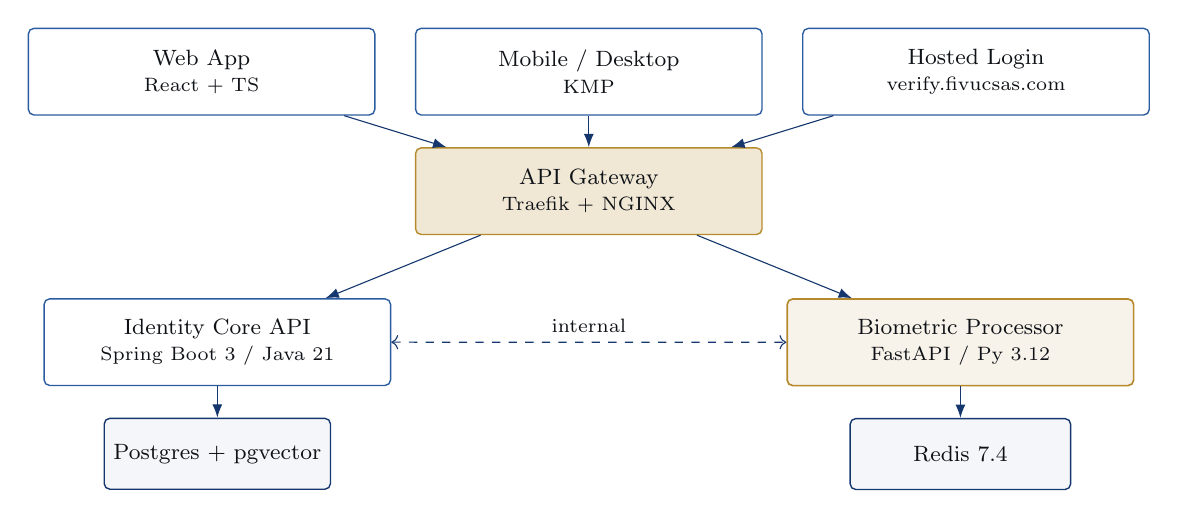
\begin{tikzpicture}[
  node distance=4mm and 5mm, every node/.style={font=\footnotesize, text=IEEEink},
  svc/.style ={draw=IEEEblue, fill=white, rounded corners=2pt,
               minimum width=4.4cm, minimum height=1.1cm, align=center, line width=0.5pt},
  ml/.style  ={draw=IEEEgold, fill=IEEEgold!10, rounded corners=2pt,
               minimum width=4.4cm, minimum height=1.1cm, align=center, line width=0.6pt},
  data/.style={draw=IEEEnavy, fill=IEEElite, rounded corners=2pt,
               minimum width=2.8cm, minimum height=0.9cm, align=center, line width=0.5pt},
  arrow/.style={-Latex, draw=IEEEnavy, line width=0.4pt}]
\node[svc] (web)     {Web App\\\scriptsize React + TS};
\node[svc, right=of web] (mobile) {Mobile / Desktop\\\scriptsize KMP};
\node[svc, right=of mobile] (widget) {Hosted Login\\\scriptsize verify.fivucsas.com};
\node[svc, below=of mobile, fill=IEEEgold!20, draw=IEEEgold] (gw) {API Gateway\\\scriptsize Traefik + NGINX};
\node[svc, below left=8mm and 0.3cm of gw] (api) {Identity Core API\\\scriptsize Spring Boot 3 / Java 21};
\node[ml,  below right=8mm and 0.3cm of gw] (bio) {Biometric Processor\\\scriptsize FastAPI / Py 3.12};
\node[data, below=of api]  (db)   {Postgres + pgvector};
\node[data, below=of bio]  (redis){Redis 7.4};
\foreach \src in {web,mobile,widget} {\draw[arrow] (\src) -- (gw);}
\draw[arrow] (gw) -- (api); \draw[arrow] (gw) -- (bio);
\draw[arrow] (api) -- (db); \draw[arrow] (bio) -- (redis);
\draw[arrow,<->,dashed] (api) -- node[above,sloped,font=\scriptsize]{internal} (bio);
\end{tikzpicture}\par\vspace{1mm}
{\footnotesize\itshape The biometric service has no public route — Docker network only, API-key gated.}}

\block{VI.~~Authentication factors}{%
\centering\footnotesize
\setlength{\tabcolsep}{4pt}\renewcommand{\arraystretch}{1.1}
\begin{tabular}{cccc}
\fcolorbox{IEEEblue}{white}{\rule{0pt}{1em}\faKey~Password} &
\fcolorbox{IEEEblue}{white}{\rule{0pt}{1em}\faEnvelope~Email OTP} &
\fcolorbox{IEEEblue}{white}{\rule{0pt}{1em}\faSms~SMS OTP} &
\fcolorbox{IEEEblue}{white}{\rule{0pt}{1em}\faClock~TOTP} \\[0.3em]
\fcolorbox{IEEEblue}{white}{\rule{0pt}{1em}\faQrcode~QR} &
\fcolorbox{IEEEgold}{IEEEgold!20}{\rule{0pt}{1em}\faSmile~Face} &
\fcolorbox{IEEEgold}{IEEEgold!20}{\rule{0pt}{1em}\faMicrophone~Voice} &
\fcolorbox{IEEEgold}{IEEEgold!20}{\rule{0pt}{1em}\faFingerprint~Print} \\[0.3em]
\fcolorbox{IEEEblue}{white}{\rule{0pt}{1em}\faUsb~WebAuthn} &
\multicolumn{3}{c}{\fcolorbox{IEEEblue}{white}{\rule{0pt}{1em}\faIdCard~NFC document (MRZ + chip)}}
\end{tabular}\par\vspace{0.4em}
{\footnotesize\itshape Gold = wrapped in active-liveness; any subset composes a tenant MFA flow.}}

\block{VII.~~Experiments and results}{%
\centering
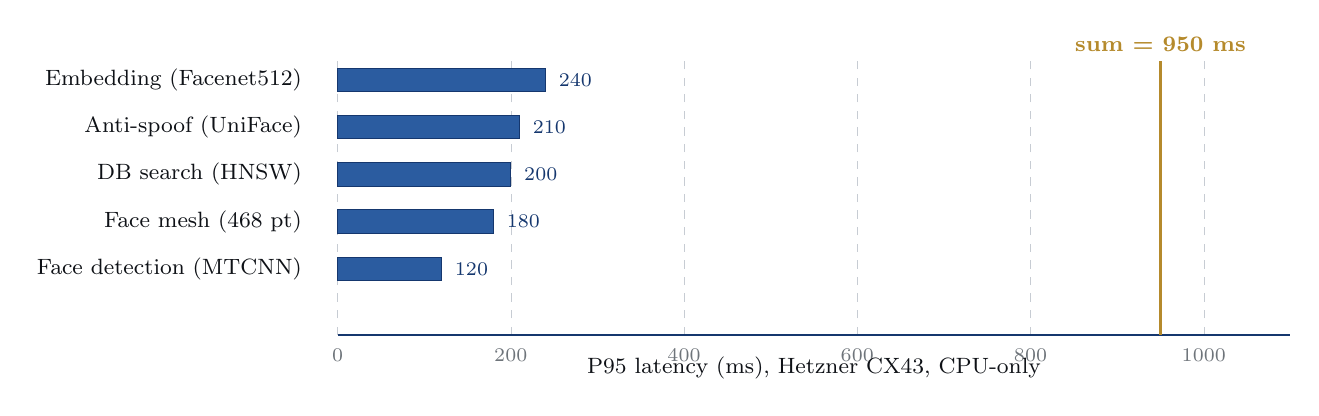
\begin{tikzpicture}[x=0.011cm, y=0.6cm,
  bar/.style={draw=IEEEnavy, fill=IEEEblue, line width=0.3pt},
  axislabel/.style={font=\footnotesize, text=IEEEink, anchor=east},
  axislabelinside/.style={font=\scriptsize, anchor=west, text=IEEEnavy},
  tickline/.style={IEEErule, dashed, line width=0.2pt}]
\foreach \x in {0,200,400,600,800,1000}{
  \draw[tickline] (\x,-0.4) -- (\x,5.4);
  \node[font=\scriptsize, anchor=north, text=IEEEgray] at (\x,-0.5) {\x};
}
\draw[IEEEnavy, line width=0.4pt] (0,-0.4) -- (1100,-0.4);
\node[font=\footnotesize, text=IEEEink] at (550,-1.1) {P95 latency (ms), Hetzner CX43, CPU-only};
\node[axislabel] at (-30,5) {Embedding (Facenet512)}; \filldraw[bar] (0,4.75) rectangle (240,5.25); \node[axislabelinside] at (240,5.0) {\,240};
\node[axislabel] at (-30,4) {Anti-spoof (UniFace)};   \filldraw[bar] (0,3.75) rectangle (210,4.25); \node[axislabelinside] at (210,4.0) {\,210};
\node[axislabel] at (-30,3) {DB search (HNSW)};       \filldraw[bar] (0,2.75) rectangle (200,3.25); \node[axislabelinside] at (200,3.0) {\,200};
\node[axislabel] at (-30,2) {Face mesh (468 pt)};     \filldraw[bar] (0,1.75) rectangle (180,2.25); \node[axislabelinside] at (180,2.0) {\,180};
\node[axislabel] at (-30,1) {Face detection (MTCNN)}; \filldraw[bar] (0,0.75) rectangle (120,1.25); \node[axislabelinside] at (120,1.0) {\,120};
\draw[IEEEgold, line width=1.0pt] (950,-0.4) -- (950,5.4);
\node[font=\footnotesize\bfseries, text=IEEEgold, anchor=south] at (950,5.4) {sum = 950 ms};
\end{tikzpicture}
\par\vspace{0.5em}
\footnotesize
\setlength{\tabcolsep}{6pt}\renewcommand{\arraystretch}{1.15}
\begin{tabular}{@{}lrr@{}}\toprule
\textbf{Quality metric}        & \textbf{Target} & \textbf{Observed} \\\midrule
Replay-attack FAR ($n\!=\!120$) & $<$\,1\,\%       & \textbf{0.0\,\%} \\
Passive-spoof AUC (internal)   & $>$\,0.95        & \textbf{0.97}    \\
Backend tests                  & green            & 633 / 633        \\
Web Vitest + Playwright        & green            & 619 + 27         \\
Mobile (KMP) units             & green            & 425 / 425        \\
\bottomrule\end{tabular}}

\block{VIII.~~Conclusion}{%
\small Production-grade, GDPR-compliant biometric authentication \emph{is} achievable on
commodity hardware when the system is decomposed along its right axis — a frozen OIDC
contract on one side, an iterating ML pipeline on the other — and when liveness is treated
as an \emph{active}, challenge-driven property rather than a single passive signal. Our
measurements indicate that the latency budget (P95 = 950~ms on a single CPU server) and the
spoof-defence profile (0\,/\,120 replay-attack false-accepts) are both within practical
deployment limits for a tenant-shared platform, with the integrity gates (1\,820+ tests, 8
ADRs, branch protection across five repositories) sufficient to keep the platform shippable
through weekly ML iteration.}

\block{IX.~~Future work}{%
\small
\begin{itemize}[leftmargin=*, itemsep=2pt, label=\textbf{--}]
\item \textbf{BYOD tenant DB.} Enterprise tenants host biometric data in their own database, schema-pinned.
\item \textbf{On-device pre-filter.} Stripped MediaPipe pipeline drops obvious non-faces before upload — bandwidth + privacy win.
\item \textbf{Cross-modal challenge.} Voice nonce + facial action to defeat audio-only deepfakes.
\item \textbf{Verifiable credentials.} W3C VCs after successful KYC for downstream-service portability.
\end{itemize}}

\block{X.~~Live demo \& references}{%
\footnotesize
\begin{minipage}[t]{0.30\linewidth}\centering
\qrcode[height=3.4cm,version=4,level=H]{https://verify.fivucsas.com}\\[1mm]
\textsc{Scan for live demo}\\
\texttt{verify.fivucsas.com}
\end{minipage}\hfill\begin{minipage}[t]{0.66\linewidth}\scriptsize\setlength{\parskip}{0pt}
\begin{enumerate}[leftmargin=*, label={[\arabic*]}, itemsep=1pt]
\item Serengil, S., Özpınar, A. \textit{LightFace / DeepFace}. IEEE ASYU, 2020.
\item Lugaresi, C.\ et al.\ \textit{MediaPipe: A Framework for Building Perception Pipelines.} arXiv:1906.08172.
\item Soukupová, T., Čech, J.\ \textit{Real-Time Eye Blink Detection using Facial Landmarks.} CVWW, 2016.
\item Wan, L.\ et al.\ \textit{Generalized End-to-End Loss for Speaker Verification.} ICASSP, 2018.
\item Yadav, S.\ et al.\ \textit{UniFace: A Unified Architecture for Face Spoofing Detection.} CVPR-W, 2023.
\end{enumerate}
\end{minipage}}

\end{columns}

% =============================================================================
% Footer
% =============================================================================
\block[bodyinnersep=2mm, bodyverticalshift=0mm]{}{%
\colorbox{IEEEnavy}{\parbox{0.985\linewidth}{\centering\color{IEEEgold}%
\vspace{2mm}\bfseries\small
\faGithub~~\texttt{github.com/Rollingcat-Software/FIVUCSAS}
\quad$\cdot$\quad
\faGlobe~~\texttt{fivucsas.com}
\quad$\cdot$\quad
\faEnvelope~~\texttt{ahmetabdullahgultekin@gmail.com}
\quad$\cdot$\quad
Marmara University \, \textbf{2026}\vspace{2mm}}}}

\end{document}
